\documentclass[a4paper]{article}
\usepackage{amsmath}
\usepackage{amsfonts}
\usepackage{amssymb}
\usepackage{graphicx}

\begin{document}

% title stuff 
\Large
 \begin{center}
Abstract for nothing\\ 

\hspace{10pt}

% Author names and affiliations
\large
Arthur Author$^1$, Cecilia CoAuthor$^2$ \\
\hspace{10pt}
\small  
$^1$) First affiliation\\
arthur.author@correspondence.email.com\\
$^2$) Second affiliation
\end{center} % end of title stuff 

% beginning of abstract
\hspace{10pt}
\normalsize
This is a simple one-page abstract template.

The first line must grab the attention of the reader!

The koala (Phascolarctos cinereus, or, inaccurately, koala bear[a]) is an arboreal herbivorous marsupial native to Australia. It is the only extant representative of the family Phascolarctidae and its closest living relatives are the wombats. The koala is found in coastal areas of the mainland's eastern and southern regions, inhabiting Queensland, New South Wales, Victoria, and South Australia. It is easily recognisable by its stout, tailless body and large head with round, fluffy ears and large, spoon-shaped nose. The koala has a body length of 60–85 cm (24–33 in) and weighs 4–15 kg (9–33 lb). Pelage colour ranges from silver grey to chocolate brown. Koalas from the northern populations are typically smaller and lighter in colour than their counterparts further south. These populations possibly are separate subspecies, but this is disputed.


\begin{figure}[h]
    \centering
    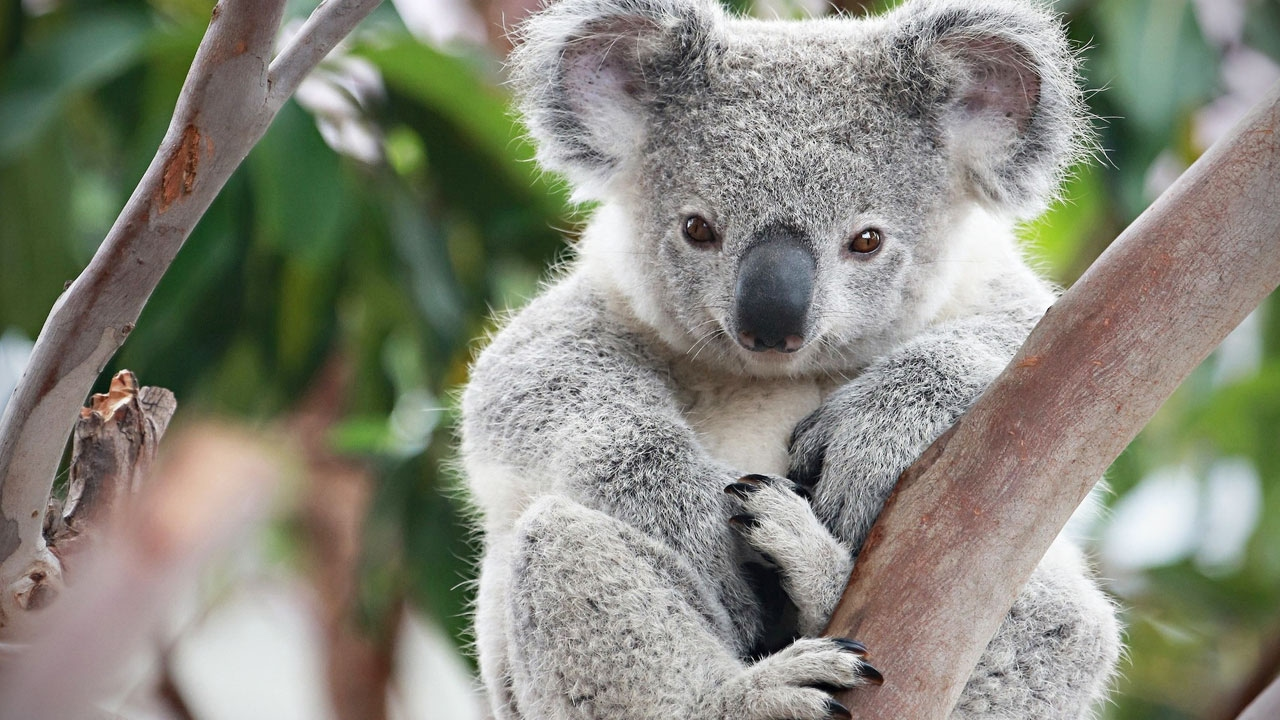
\includegraphics[width=0.6\textwidth]{figs/koala.jpg}
    \caption{A koala}
    \label{fig:koala}
\end{figure}
 
As you can see in figure \ref{fig:koala}, the koala is an arboreal herbivorous marsupial.


\end{document}